\chapter{Introduction}
\label{chap:introduction}

\section{{Plasma Modulated Plasma Accelerator}}
\label{sec:intro-motivation}
A plasma can be formed by ionising a gas target using a high-intensity, short (10 fs) laser pulse. 
The interaction of the laser pulse with the plasma can form accelerating structures with field 
strengths of the order of 100 GV/m. In a laser-wakefield accelerator scheme (LWFA), these accelerating structures may be used 
to achieve electron energies in the order of 100s MeV to GeV \cite{esarey2009}. Such schemes may lead to the production of compact, low cost
electron sources with applications such as light source generation \cite{geddes2017}, QED experiments \cite{los2025}, radiobiology studies
 \cite{mcanespie2024}, and probing fundamental plasma 
physics \cite{balcazar2025}.

LWFA schemes are currently limited by the repititon rates of their laser systems, most commonly $\lessapprox$ 10 Hz with Ti:sapphire lasers. 
The University of Oxford's Laser Plasma Accelerator Group (LPAG) is working with collaborators on the plasma-modulated plasma accelerator (P-MoPA)
project to address this \cite{jakobsson2021,alejo2022,vandewetering2023,vandewetering2024,ross2024}. The project aims to use thin-disk lasers
with high repititon rates ($\sim$ 1 kHz) to drive a LWFA electron source. The pulse duration of such lasers is too long too drive a LWFA, so
the following scheme is used to create a pulse-train (see Figure~\ref{fig:pmopa}): A short, low-energy seed-pulse is co-propagated with a long drive-pulse through
a modulator stage containing a gas. The seed-pulse ionises the gas and drives a low-intensity plasma wave that modulates the drive-pulse,
producing side-bands in its spectrum. A compressor then removes the phase on these side-bands, converting the picosecond pulse into a train
of short pulses spaced temporally by the plasma period. This pulse train can then be directed into a second plasma stage of the same density,
resonantly exciting a wakefield into which electrons can be injected and subsequently accelerated. This modulation-compression process is
sensitive to the drive-pulse's spatio-spectral content; any spatio-spectral couplings would vary the modulation across the pulse's profile and
degrade the resulting pulse-train, weakening the pulse-train's ability to drive a wakefield and leading to unstable electron acceleration.
The characterisation of spatio-spectral couplings in the thin-disk lasers used in the P-MoPA project is thus essential for the project's success.

\begin{figure}[tbp]
    \centering
    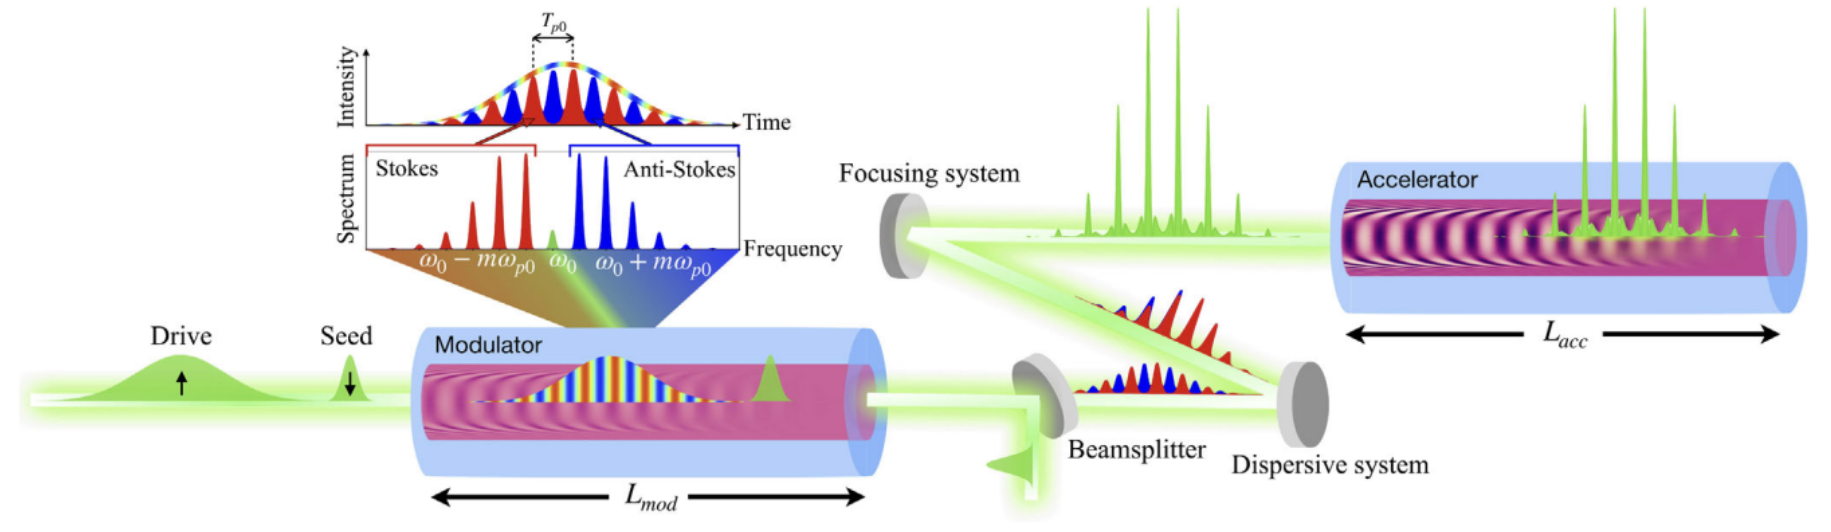
\includegraphics[width=\textwidth]{figures/pmopa.png}
    \caption[The Plasma Modulated Plasma Accelerator (P-MoPA) scheme.]{The Plasma Modulated Plasma Accelerator (P-MoPA) scheme. Reproduced from \cite{jakobsson2021}.}
    \label{fig:pmopa}
\end{figure}


\section{Angular and Spatial Chirp}
\label{sec:intro-background}

\subsection{Chirped Pulse Amplification}
\label{sec:intro-cpa}

Prior to Gérard Mourou and Donna Strickland's invention of chirped pulse
amplification (CPA) \cite{strickland1985}, for which they were awarded the Nobel Prize in Physics
in 2018, it was extremely challenging to produce ultrashort laser pulses with
enough intensity
for modern LWFA without damaging the optical equipment and introducing
non-linear effects. CPA avoids these issues through a staged amplification
procedure (see Figure~\ref{fig:cpa}): An ultrashort, low-amplitude pulse enters
a pulse stretcher, composed of two identical parallel diffraction gratings. 
This stretches the pulse temporally, reducing its intensity without loss of
energy. The pulse is subsequently amplified then directed through a pulse 
compressor, similar to the pulse stretcher, which compresses the pulse back to 
its original duration. The result is a high-intensity ultrashort pulse, but 
crucially this intensity is only reached post-compressor, leaving all previous
optical components unharmed.

As with most real optical systems, CPA systems are highly sensitive to
misalignments. In particular, a relative misalignment between the two gratings
of the stretcher or the compressor, or a mismatch between the dispersive properties
of the stretcher and the compressor, may produce spatio-spectral couplings in the 
pulse. One such coupling is known as \emph{angular chirp}, a correlation between 
the angle
of propagation $\theta$ and wavelength $\lambda$ within a pulse of finite bandwidth. 
When an angularly chirped pulse propagates over a finite distance, it acquires
\emph{spatial chirp}, a correlation between position $x$ along an arbitrary 
transverse axis across a pulse 
and wavelength $\lambda$.

\begin{figure}[tbp]
    \centering
    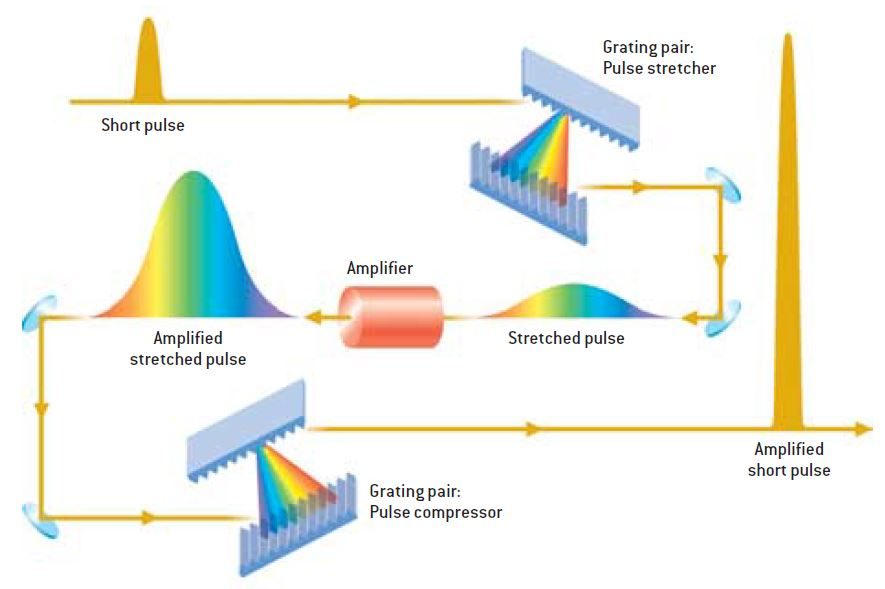
\includegraphics[width=\textwidth]{figures/CPA.jpg}
    \caption[Illustration of Chirped Pulse Amplification (CPA).]{Illustration of
     Chirped Pulse Amplification (CPA). Reproduced from \cite{cuos2026}.}
    \label{fig:cpa}
\end{figure}

% TODO: Brief CPA primer (stretch -> amplify -> compress) -- only as much as
% needed to motivate why the amplified pulse can pick up spatio-spectral
% coupling. See presentation slide 5.

\subsection{Angular-to-Spatial Chirp Conversion at Focus}
\label{sec:intro-angular-to-spatial}

\begin{figure}[tbp]
    \centering
    \begin{subfigure}[b]{0.48\textwidth}
        \centering
        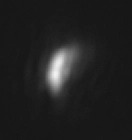
\includegraphics[width=\textwidth]{figures/lens_spatial_chirp.jpg}
        \caption{Lens focus}
        \label{fig:lens-focus}
    \end{subfigure}
    \hfill
    \begin{subfigure}[b]{0.48\textwidth}
        \centering
        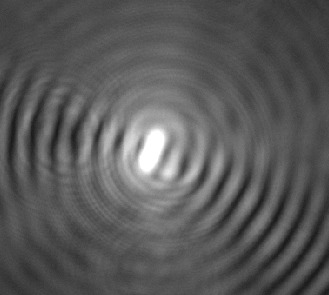
\includegraphics[width=\textwidth]{figures/axicon_spatial_chirp.jpg}
        \caption{Axicon focus}
        \label{fig:axicon-focus}
    \end{subfigure}
    \caption[Spatially chirped lens and axicon foci.]{
        Spatially chirped foci resulting from angularly
    chirped incident pulses. Images courtesy of Alexander Harrison.}
    \label{fig:lens_and_axicon_foci}
\end{figure}

A useful property of the converging lens is the conversion between angular and spatial
information at its focal plane. In particular, any collimated plane wave 
incident on an ideal thin lens of focal length $f$ is, in the paraxial 
approximation, focussed to a transverse position $x$ on the lens' 
back focal plane proportional to its angle of incidence $\theta$:
\begin{equation}
    x=f\theta.
    \label{eq:fourier_lens}
\end{equation}
Consequently, if the incident pulse is angularly chirped, 
meaning $\theta$ is spectrally dependent, the transverse position $x$ of the 
resulting focal spot
also becomes spectrally dependent, meaning it is spatially chirped. The result is 
a focal spot that is stretched along an arbitrary transverse axis, as
opposed to a typical circular focal spot. (see Figure
\ref{fig:lens_and_axicon_foci}).
 
Differentiating Equation \ref{eq:fourier_lens} with respect
to wavelength $\lambda$:
\begin{equation}
    \frac{dx}{d\lambda}=f\frac{d\theta}{d\lambda}.
    \label{eq:ang_to_spat_chirp}
\end{equation}
The derivative $\zeta\equiv\frac{dx}{d\lambda}$ is known as \emph{spatial dispersion},
corresponding to a pulse's spectrally dependent transverse position $x(\lambda)$, and
is the conventional metric used for describing spatial chirp throughout this 
project. Another common metric used for describing spatial chirp is known as 
the frequency gradient, $\frac{d\omega}{dx}$, corresponding to a pulse's 
transverse-positionally dependent angular frequency $\omega(x)$. While these
parametarisations both describe spatial chirp, they are not simply reciprocals of
each other \cite{gu2004}. Spatial dispersion is used throughout this project because
of its convenient relationship with the angular dispersion $\frac{d\theta}{d\lambda}$
that produces it. Wavelength is chosen as the spectral unit throughout this project
due to its direct relationship with the diffraction angle of optical gratings.



% TODO: Derive/explain how angular chirp d(theta)/d(lambda) upstream of a
% focussing optic becomes spatial chirp dx/d(lambda) at focus. See
% presentation slides 6-7 (lens vs axicon focus comparison).

\subsection{Consequences for the Plasma Wave}
\label{sec:intro-consequences}

% TODO: Spatial chirp -> elongated focal spot / longer pulse duration /
% reduced intensity; angular chirp -> pulse front tilt -> asymmetric drive
% of the plasma wave. See presentation slide 8 ("Why Should You Care?").

\section{Measuring Angular Chirp}
\label{sec:intro-measuring}

% TODO: Motivate the imaging-spectrometer approach as the measurement
% technique chosen (transition from "how do we measure this" to "here is
% the instrument we built" -- bridges into chapter 2). See presentation
% slide 9.

\section{Project Objectives}
\label{sec:intro-objectives}

% TODO: State the concrete goals -- design and deploy an imaging
% spectrometer, build the acquisition/calibration/preprocessing/analysis
% software pipeline, build a GUI, and use it to test a known spatial-chirp
% source (glass windows).

\section{Report Outline}
\label{sec:intro-outline}

% TODO: One short paragraph per remaining chapter (Optical Design,
% Calibration, Analysis Pipeline, Graphical User Interface, Experimental
% Design, Results, Discussion, Conclusions).
